% 
\RequirePackage{amsmath}
\documentclass[a4paper]{article}
\usepackage{Sweave}
\usepackage[margin=0.5in]{geometry}
\usepackage{enumitem}
\usepackage{float}
\usepackage[usenames,dvipsnames]{color}

\usepackage{titlesec}% http://ctan.org/pkg/titlesec
\titleformat{\section}%
  [hang]% <shape>
  {\normalfont\bfseries\Large}% <format>
  {}% <label>
  {0pt}% <sep>
  {}% <before code>
\renewcommand{\thesection}{}% Remove section references...
\renewcommand{\thesubsection}{\arabic{subsection}}%... from subsections

\title{Module 1 - Basic Probability and Statistics}
\author{Pawel Chilinski}

\begin{document}
\input{PawelChilinski_module1_exercises-concordance}
\maketitle
\section{Part 1 - Probability}

\subsection{Find a distribition function $F_x(x) = P(X \leq x)$, $x \in R$ of
random variable X.}

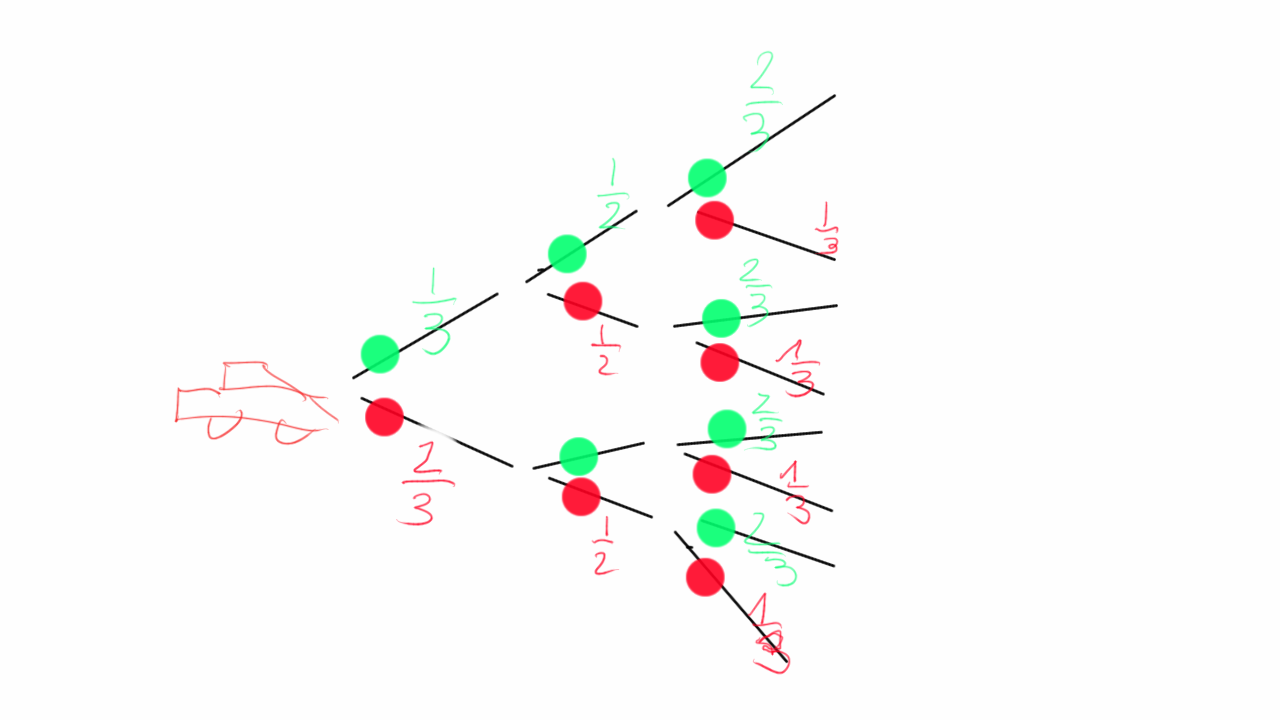
\includegraphics{car.png}

X - random variable equal to a number of times the driver had to stop on his way
due to red light in crossroads.
\\

$P(X=0)=\frac{1}{3}\cdot\frac{1}{2}\cdot\frac{2}{3}=\frac{1}{9}$
\\

$P(X=1)=\frac{2}{3}\cdot\frac{1}{2}\cdot\frac{2}{3}+\frac{1}{3}\cdot\frac{1}{2}\cdot\frac{2}{3}+\frac{1}{3}\cdot\frac{1}{2}\cdot\frac{1}{3}
=\frac{7}{18}$
\\

$P(X=2)=\frac{2}{3}\cdot\frac{1}{2}\cdot\frac{2}{3}+\frac{1}{3}\cdot\frac{1}{2}\cdot\frac{1}{3}+\frac{2}{3}\cdot\frac{1}{2}\cdot\frac{1}{3}=
\frac{7}{18}$
\\

$P(X=3)=\frac{2}{3}\cdot\frac{1}{2}\cdot\frac{1}{3}=\frac{1}{9}$

\[ F_x(x) = \left\{ 
  \begin{array}{l l}
    0 \quad x<0\\
    1/_9 \quad 0\leq x <1\\
    1/_2 \quad 1\leq x <2\\
    8/_9 \quad 2\leq x <3\\
    1 \quad 3\leq x}
  \end{array} \right\]
  
\subsection{Find the probability that a person randomly chosen from the
population has IQ}

\begin{enumerate}[label=\emph{\alph*})]
\item  above 130
\begin{Schunk}
\begin{Sinput}
> 1-pnorm(130,mean=100,sd=15)	
\end{Sinput}
\begin{Soutput}
[1] 0.02275013
\end{Soutput}
\end{Schunk}
\item between 100 and 120
\begin{Schunk}
\begin{Sinput}
> pnorm(120,mean=100,sd=15)-pnorm(100,mean=100,sd=15)
\end{Sinput}
\begin{Soutput}
[1] 0.4087888
\end{Soutput}
\end{Schunk}
\end{enumerate}

\subsection{A pair of random variables (X, Y) has a joint discrete distribution}

\begin{enumerate}[label=\emph{\alph*})]
\item  marginal distributions
\begin{table}[H]
\begin{center}
  \begin{tabular}{ l | l l l | l}
    X\textbackslash Y & -1 & 0 & 1 & \textcolor{Emerald}{$p_x$} \\ \hline
    0 & 0.1 & 0.1 & 0 & \textcolor{Emerald}{0.2}\\
    1 & 0.2 & 0.2 & 0.1 & \textcolor{Emerald}{0.5}\\
    2 & 0.1 & 0.1 & 0.1 & \textcolor{Emerald}{0.3}\\
    \hline
    \textcolor{blue}{$p_y$} & \textcolor{blue}{0.4} & \textcolor{blue}{0.4} &
    \textcolor{blue}{0.2} & \\
  \end{tabular}
\end{center}
\end{table}
\item Calculate P(X > 2Y)
\\

P(X=x, Y=y) := P(x,y)
\\

P(X > 2Y)=P(0,-1)+P(1,-1)+P(1,0)+P(2,-1)+P(2,0)=0.1+0.2+0.2+0.1+0.1=0.7
\\

\item Are random variables X and Y independent? Calculate Cov(X,Y) and Cor(X,Y)
\\

They are not independent because $P(0,-1)=0.1 \neq P(X=0)\cdot P(Y=-1)=0.2\cdot 0.4 = 0.08$
\\

\begin{Schunk}
\begin{Sinput}
> EX <- 0.2 * 0 + 0.5 * 1 + 0.3 * 2
> EX
\end{Sinput}
\begin{Soutput}
[1] 1.1
\end{Soutput}
\begin{Sinput}
> EY <- 0.4 * -1 + 0.4 * 0 + 0.2 * 1
> EY
\end{Sinput}
\begin{Soutput}
[1] -0.2
\end{Soutput}
\begin{Sinput}
> E_XY <- 0.2 * 1 * -1 + 0.1 * 1 * 1 + 0.1 * 2 * -1 + 0.1 * 2 * 1
> E_XY
\end{Sinput}
\begin{Soutput}
[1] -0.1
\end{Soutput}
\begin{Sinput}
> var_X <- 0.2*(0-EX)^2 + 0.5*(1-EX)^2 + 0.3*(2-EX)^2
> var_X
\end{Sinput}
\begin{Soutput}
[1] 0.49
\end{Soutput}
\begin{Sinput}
> var_Y <- 0.4*(-1-EY)^2 + 0.4*(0-EY)^2 + 0.2*(1-EY)^2
> var_Y
\end{Sinput}
\begin{Soutput}
[1] 0.56
\end{Soutput}
\begin{Sinput}
> cov_XY <- E_XY-EX*EY
> cov_XY
\end{Sinput}
\begin{Soutput}
[1] 0.12
\end{Soutput}
\begin{Sinput}
> cor_XY <- cov_XY/sqrt(var_X*var_Y)
> cor_XY
\end{Sinput}
\begin{Soutput}
[1] 0.2290811
\end{Soutput}
\end{Schunk}
\item Find conditional distribution
\\

$P(X|Y=-1)=\frac{P(X,Y=-1)}{P(Y=-1)}$
\begin{table}[H]
\begin{center}
  \begin{tabular}{ l | l l l}
    X|Y=-1 & 0 & 1 & 2 \\ \hline
      &   &   &   \\
      & $\frac{0.1}{0.4}$ & $\frac{0.2}{0.4}$ & $\frac{0.1}{0.4}$ \\ 
  \end{tabular}
  \quad
  =
  \quad
  \begin{tabular}{ l | l l l}
    X|Y=-1 & 0 & 1 & 2 \\ \hline
      & 0.25 & 0.5 & 0.25 \\ 
  \end{tabular}
\end{center}
\end{table}
\\

$P(Y|X=0)=\frac{P(Y,X=0)}{P(X=0)}$
\begin{table}[H]
\begin{center}
  \begin{tabular}{ l | l l l}
    Y|X=0 & -1 & 0 & 1 \\ \hline
      &   &   &   \\
      & $\frac{0.1}{0.2}$ & $\frac{0.1}{0.2}$ & $\frac{0}{0.2}$ \\ 
  \end{tabular}
  \quad
  =
  \quad
  \begin{tabular}{ l | l l l}
    Y|X=0 & -1 & 0 & 1 \\ \hline
      & 0.5 & 0.5 & 0 \\ 
  \end{tabular}
\end{center}
\end{table}
\end{enumerate}

\subsection{Using central limit theorem find an approximate distribution of the time in which a cyclist covers 50km of the route}
\\

The expected value of the time that cyclist needs to complete 1km is:
$EX=\frac{1.4+1.8}{2}=1.6$ min
\\
The variance of the time that cyclist needs to complete 1km is:
$\sigma_{x}^2=\frac{(1.8-1.4)^2}{12}=$ 0.0133 
\\

So according to CLT the we can model the time needed to complete 50 km route by
normal distribution
N(50\cdot1.6,50\cdot0.0133)=N(80,0.665).

\section{Part 2 - Statistics}
\setcounter{subsection}{4}
\subsection{Find 95\% confidence interval for the expected value of a textbook
price}
\\

Because $\frac{\bar{P_n} - \mu}{\frac{\sigma}{\sqrt{n}}}  \sim N(0,1)$ then
\begin{Schunk}
\begin{Sinput}
> mu_p <- 28.4
> sd_p <- 4.75
> n <- 50
> conf_interval_0_95 <- c(mu_p-qnorm(0.975)*sd_p/sqrt(n) , mu_p + qnorm(0.975)*sd_p/sqrt(n))
> conf_interval_0_95
\end{Sinput}
\begin{Soutput}
[1] 27.08339 29.71661
\end{Soutput}
\end{Schunk}
\\

\subsection{Perform a statistical test to validate their hypothesis, with significance level equal to 0.05.}
\\

$H_0 : fraction = 0.25$
\\
$H_1 : fraction \neq 0.25$ 
\\

Here we deal with example of binomial distribution. And we standardize fraction
assuming $H_0$ holds: 
\begin{Schunk}
\begin{Sinput}
> n <- 400
> frac_est <- 79/400
> frac_0 <- 0.25
> frac_standardized <- (p_est-p_0)/sqrt(p_est*(1-p_est)/n)